\section{Application to Thermal Protection Systems}

In this section, the proposed PIROM approach is applied to modeling a four-layered hypersonic TPS with unknown contact resistances, and is compared against a representative physics-based model, i.e., FEMs, and data-driven surrogate model, i.e., a neural ordinary differential equation (NODE) model. The performance of the models is assessed in terms of their ability to infer the TCRs, and to predict the transient temperature dynamics under varying boundary conditions and material properties. The configuration of the TPS, problem parametrization, optimal model design for inference, and numerical results are presented next.

\subsection{Problem Description and Parametrization}


\subsection{Model Selection}



\subsubsection{One-Dimensional Finite-Element Model}

In Section~\ref{sec:1dfem}, the 1D-FEM was introduced as utilizing linear basis functions (LBFs). These LBFs have favorable behavior when put in weak form, yielding simple stiffness and mass matrices that captures the heat transfer within material blocks and the imperfect interfaces between said blocks. However, the 1D-FEM also has the added benefit of being a first-order model; consequently, by leveraging the pair of LBFs on each side of a respective material block, the temperature at any given sensor position within the block can be easily computed via a weighted average. 

Consider the example presented in Fig.~\ref{fig:lbf_demo}, where each of the sensors are perturbed from their respective interfaces by distance $\delta$. The temperature of $z_1^{\text{HF}}$ when the temperatures on the left and right side of the first material block are $u_l$ and $u_r$ respectively is then given by
\begin{equation}
    u = u_l \cdot \frac{L-\delta}{L} + u_r \cdot \frac{\delta}{L}
\end{equation}
where $L$ is the thickness of the material block in question. By computing the weighted average of every sensor with respect to the two edge temperatures on either side, the sensor temperatures can be found regardless of the distance $\delta$ in which they are perturbed.

To examine the ability of the 1D-FEM in inferring the gap TCRs, the model will be tested in a range of experiments with two varying parameters: noise level and perturbation distance, $\delta$. For varying noise level, the high fidelity sensor readings will be injected with random Gaussian noise to corrupt the temperature signals. These sensors will then be denoised using a weak form kernel ridge regression framework \cite{kreider2026} prior to TCR training; the subsequent denoising should clean and smooth the signal, but may introduce some biases that could interfere with the inferred conductances. In response, several seeds will be evaluated for each experiment (i.e., noise level and sensor placement) --- allowing for the analysis of the overall behavior of adding noise to the system, and neglecting the erratic residue of any single seed performance. Doing so should make the evolution of TCR inference error with respect to increasing noise level clear. 

Additionally, six different sensor perturbation distances will be evaluated, or $\delta_i$ for $i=1,2,\dots,6$. These perturbations range from 0\% - 20\% of the block length $L$, with higher $i$ values corresponding to more extreme displacements of the sensors away from their respective interfaces. By sweeping a range of sensor positions from perfect to extremely perturbed placement, the trend of how conductance inference error is affected by moving the sensors away from their interfaces will be clear. 

The mean error across the ensemble is presented in Fig.~\ref{fig:cond_mean}, where the 1D-FEM model occupies the first row. It is immediately apparent that the dominant error mode of TCR inference is the sensor position, as error significantly increases as the sensor is perturbed further away from the interface. Such behavior is likely a byproduct of the LBFs, which can only accurately predict the sensor temperature readings within a small distance of the interfaces. Most of this error originates from the sensor in Acusil, whose low conductance produces an asymptotic curve that is difficult to approximate with LBFs alone. Similarly, the error increases slightly as the noise level increases, an artifact of the small biases introduced by the noise/denoise framework that shift the inferred TCR solution.

The standard deviation error for the same ensemble is illustrated in Fig.~\ref{fig:cond_std}, where the noise level is a major source of variation. Observe the negligible STD of the no-noise case where all ensembles produce essentially identical solutions, while the moderate- and high-noise cases produce steadily increasing STDs as a result of the denoising. Since more extreme noises may introduce similarly behaving biases, different seeds can produce greatly varying conductance errors. Note that at further sensor positions the perturbation error dominates the that of the noise significantly, resulting in less STD as the sensor moves further and further away (but still higher mean error). 

To summarize, the 1D-FEM performs exceptionally well when the sensor is near-perfectly placed with no significant noise. However, at large displacements or high noise levels this error rises quite significantly, an artifact of both the diminishing accuracy of the LBFs and the biases introduced by the denoising algorithm. 


\begin{figure}[htbp]
    \centering
    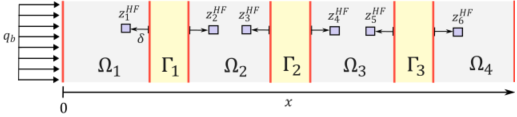
\includegraphics[width=0.8\linewidth]{figs/modeling/1D_FEM_Offset.png}
    \caption{Experimental setup with arbitrary sensor displacement, $\delta$, applied to each of the six sensors.}
    \label{fig:lbf_demo}
\end{figure}

\begin{enumerate}
    \item Discuss sensor placement and how it is done for this specific system (i.e. LBFs)
    \item Tradeoff for $C$ vs $\delta$ vs $\mathrm{SNR}$ (however, this might be best placed in the appendix with the main takeaways in the main document)
\end{enumerate}










\subsubsection{Lumped Capacitance Model}

The lumped capacitance models (LCMs) from Section~\ref{sec:lcm}, which are contrarily based in a finite-volume model, are rooted differently. Rather than leveraging LBFs to formulate a first-order model like the 1D-FEM, the LCMs operate as a zeroth-order model; that is, the only known values are the average block temperatures, and all other information must be subsequently deduced. Consequently, the approach of computing the temperature is more elaborate, consisting of recomputing effective conductances. 

Consider the demonstrative experiment presented in Fig.~\ref{fig:lcm_demo}, where a pair of sensors on either side of an interface are shown. By adjusting the $\delta$ sensor position, the effective resistance across a gap can be computed --- by moving the sensor away from the interface, the calculation must not only account for the gap resistance, but also the resistance of the block between the sensor and the interface. Consequently, the corrected resistance ensures the flux is accurate, correcting the temperatures jump in temperature across the gap and ensuring the inferred conductance is accurate. 

For perfect sensor placement, the resistance across the gap is simply $R_{x_i}$. However, as the sensor is moved away from the interface, one must account for the resistances in either material block for a proper IHCP. Thus, it is imperative to adjust the temperature jump across the gap; as heat flux is constant across the material blocks and gap interfaces, this is quite intuitive. Consider
\begin{equation}
    q = \frac{\Delta T}{R_{\text{eff}}}
\end{equation}
where the flux is given by the temperature jump across a gap with effective resistance $R_\text{eff}$. Since the flux across the interface itself will be equal to the flux through the material block and gap, the temperature difference at the new sensor positions can be computed through their relation. For $\Delta \theta$ and $\Delta z$ representing the temperature difference for the perfect and perturbed sensor placement respectively, the relation is
\begin{equation}
    \frac{\Delta z}{R_{x_1} + R_1^- + R_1^+} = \frac{\Delta \theta}{R_{x_i}} 
\end{equation}
which yields the corrected temperature jump as
\begin{equation}
    \Delta z = \Delta \theta \left[1+\frac{R_1^- + R_1^+}{R_{x_i}}\right]
\end{equation}
This framework shows how finite-volume methodology can be leveraged to compute the temperatures at the new sensor locations. As an added sanity check, if the sensor placement is perfect, $R_i^-=R_i^+=0$, which would yield $\Delta z = \Delta \theta$.

Similarly to the 1D-FEM, the LCM will be examined on its ability to infer the gap TCRs. However, in addition to testing the noise levels and perturbation distance, the refinement of the model will also be analyzed. For instance, the most coarse LCM can have four elements, one for each block --- this is denoted as LCM 4. However, the number of elements can be greater than four as well. Consider an LCM with six elements (i.e., LCM 6) which can be distributed to the four material blocks. A naive way of handling this is to place the two extra elements in random blocks, but a more structured framework is to place both extra blocks in Acusil. As Acusil has a significantly smaller conductivity --- and thus a larger temperature gradient --- the zeroth-order approximation would be the most inadequate here. Therefore, for LCM models with five or more elements, the extra elements will be isolated to the first material block where they can improve tracking of the Acusil temperature profile near the sensor. To supplement this framework, a spline can also be fit for the two elements nearest to the sensor in the Acusil layer, similar to flux reconstruction. This way the component averages can be further leveraged to improve sensor temperature approximations as $\delta$ perturbs the sensor with respect to the elements. 

By varying the noise level, sensor position, and LCM discretization, the mean errors in TCR inference can be generated as shown in Fig.~\ref{fig:cond_mean}. Observe that LCM 4 performs roughly the same as the 1D-FEM in terms of sensor placement, likely due to its similar discretization; without more elements in the Acusil layer, the temperature approximation of the sensor further from the interface is inadequate, producing a poorly inferred conductance value. However, for finer discretized models (e.g., LCM 5 and so on), the error is much smaller and more uniform, an artifact of the better sensor approximation. However, between these finely discretized models, there is not much improvement; that is, there is no real improvement from putting more than two elements in Acusil, as these two already map the temperature gradient quite well. Finally, in terms of noise level, the errors are similar to 1D-FEM for all models --- error increases slightly as the noise level increases, likely due to the biases that get introduced through the noise/denoise workflow. 

Similarly, the standard deviations for the error in inferred conductances is shown in Fig.~\ref{fig:cond_std}. Similar to 1D-FEM, the standard deviation increases as a function of noise level, with moderate noise having higher deviation than no noise, and high noise more than both. However, contrarily to the 1D-FEM and LCM 4, the finely discretized models have more uniform standard deviations. This is likely due to their overall low error, which maintains the noise level as a dominant error mode as opposed to the sensor placement in the coarser models. 

\begin{figure}[htbp]
    \centering
    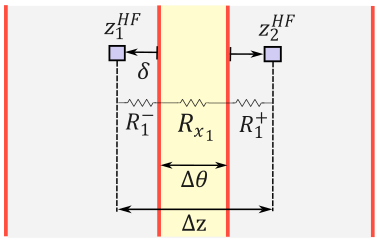
\includegraphics[width=0.4\linewidth]{figs/modeling/LCM_Demo.png}
    \caption{Demonstrative example of an arbitrary sensor displaced from its respective interface position, showing the varying effective resistance with increasing $\delta$.}
    \label{fig:lcm_demo}
\end{figure}

\begin{enumerate}
    \item Discuss sensor placement and how it is done for this specific system (i.e. moving indices in FEM)
    \item Tradeoff for $C$ vs $\delta$ vs $\mathrm{SNR}$ (however, this might be best placed in the appendix with the main takeaways in the main document)
\end{enumerate}




\subsubsection{Remarks}

With the previous analysis of the 1D-FEM and LCMs, the best choice in training for PIROM is clearly LCM 5. In Fig.~\ref{fig:cond_mean}, it is apparent that the finer models have constantly negligible error regardless of sensor position. And while there is no further improvement in error for even finer models (e.g., LCM 6-8), there is a considerable increase in runtime effort. LCM 5, which only has 5 elements, remains computationally tractable while still displaying the benefit of additional elements in Acusil. Furthermore, LCM 5 displays steady behavior across noise levels, and only sees a comparable rise in standard deviation with moderate noise compared to the other models. 

Finally, the moderate noise case is the best case to train the PIROM on, since it permits for the analysis of the effects of noise on the system while maintaining a noise intensity similar to that of real sensors. Additionally, it shows the effects of noise while still being physical; the increase in mean and deviation error rise slightly as expected, but they are still tractable for a solver. While the models were able to handle the high noise case, the intensity is quite a bit more extreme than is reasonable and is meant as more of a demonstrative example of the limitations of the model and the trend of the models with gradually increasing noise. 

\begin{figure}[htbp]
    \centering
    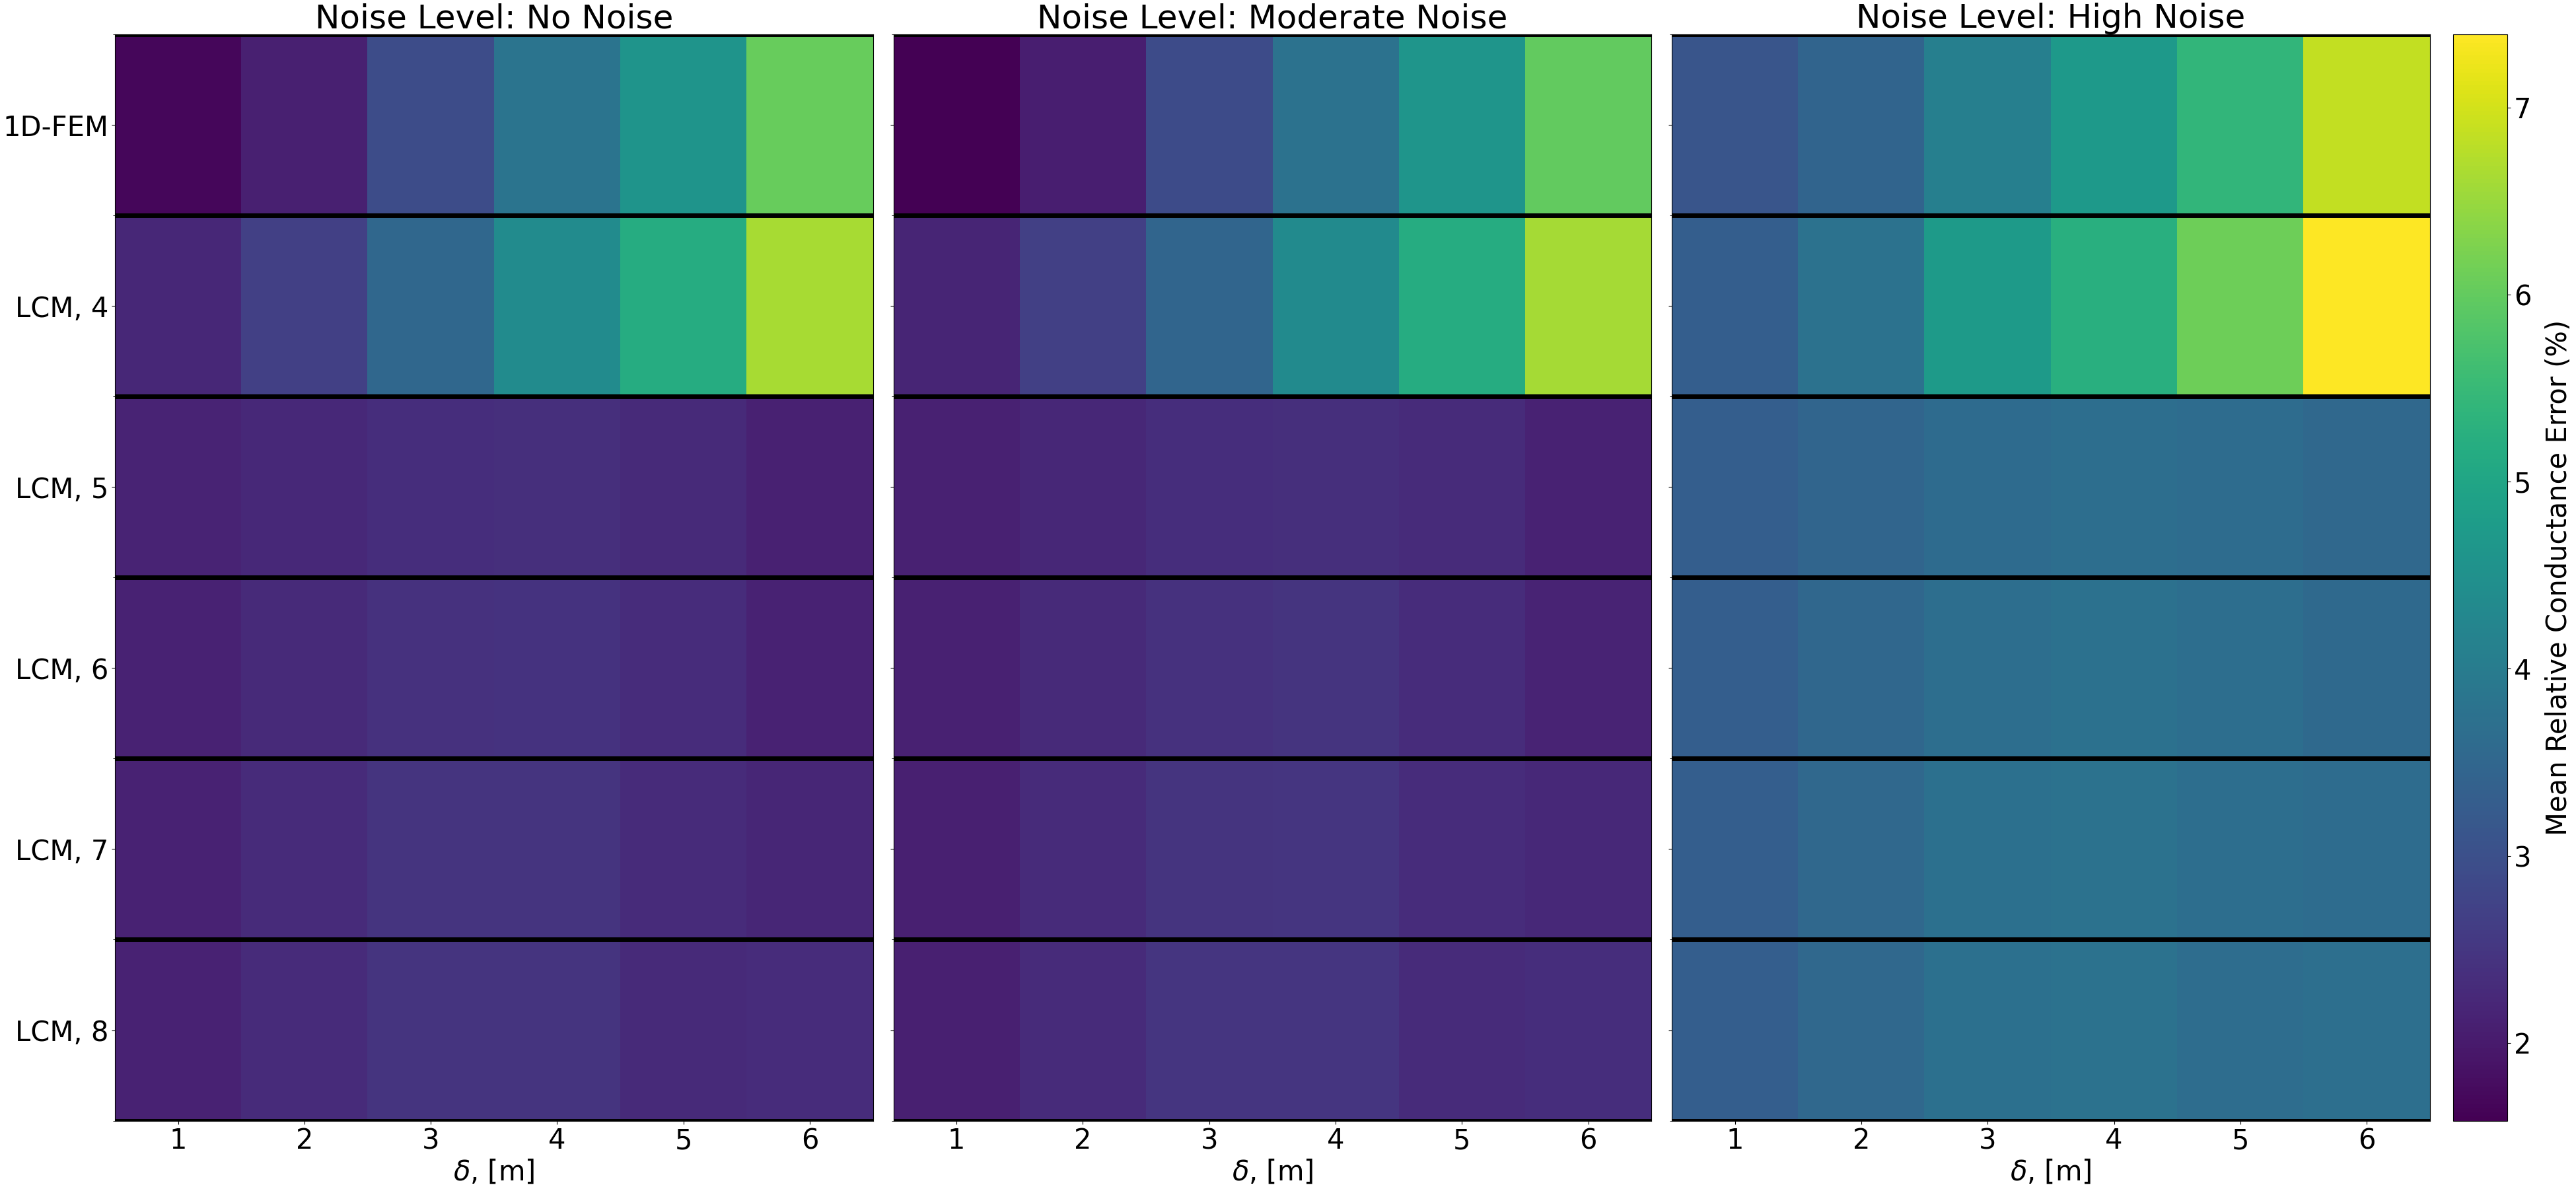
\includegraphics[width=0.99\textwidth]{./figs/results/cond_mean.png}
    \caption{Mean relative error of the inferred conductance values across a range of experiments and model selections. }
    \label{fig:cond_mean}
\end{figure}

\begin{figure}[htbp]
    \centering
    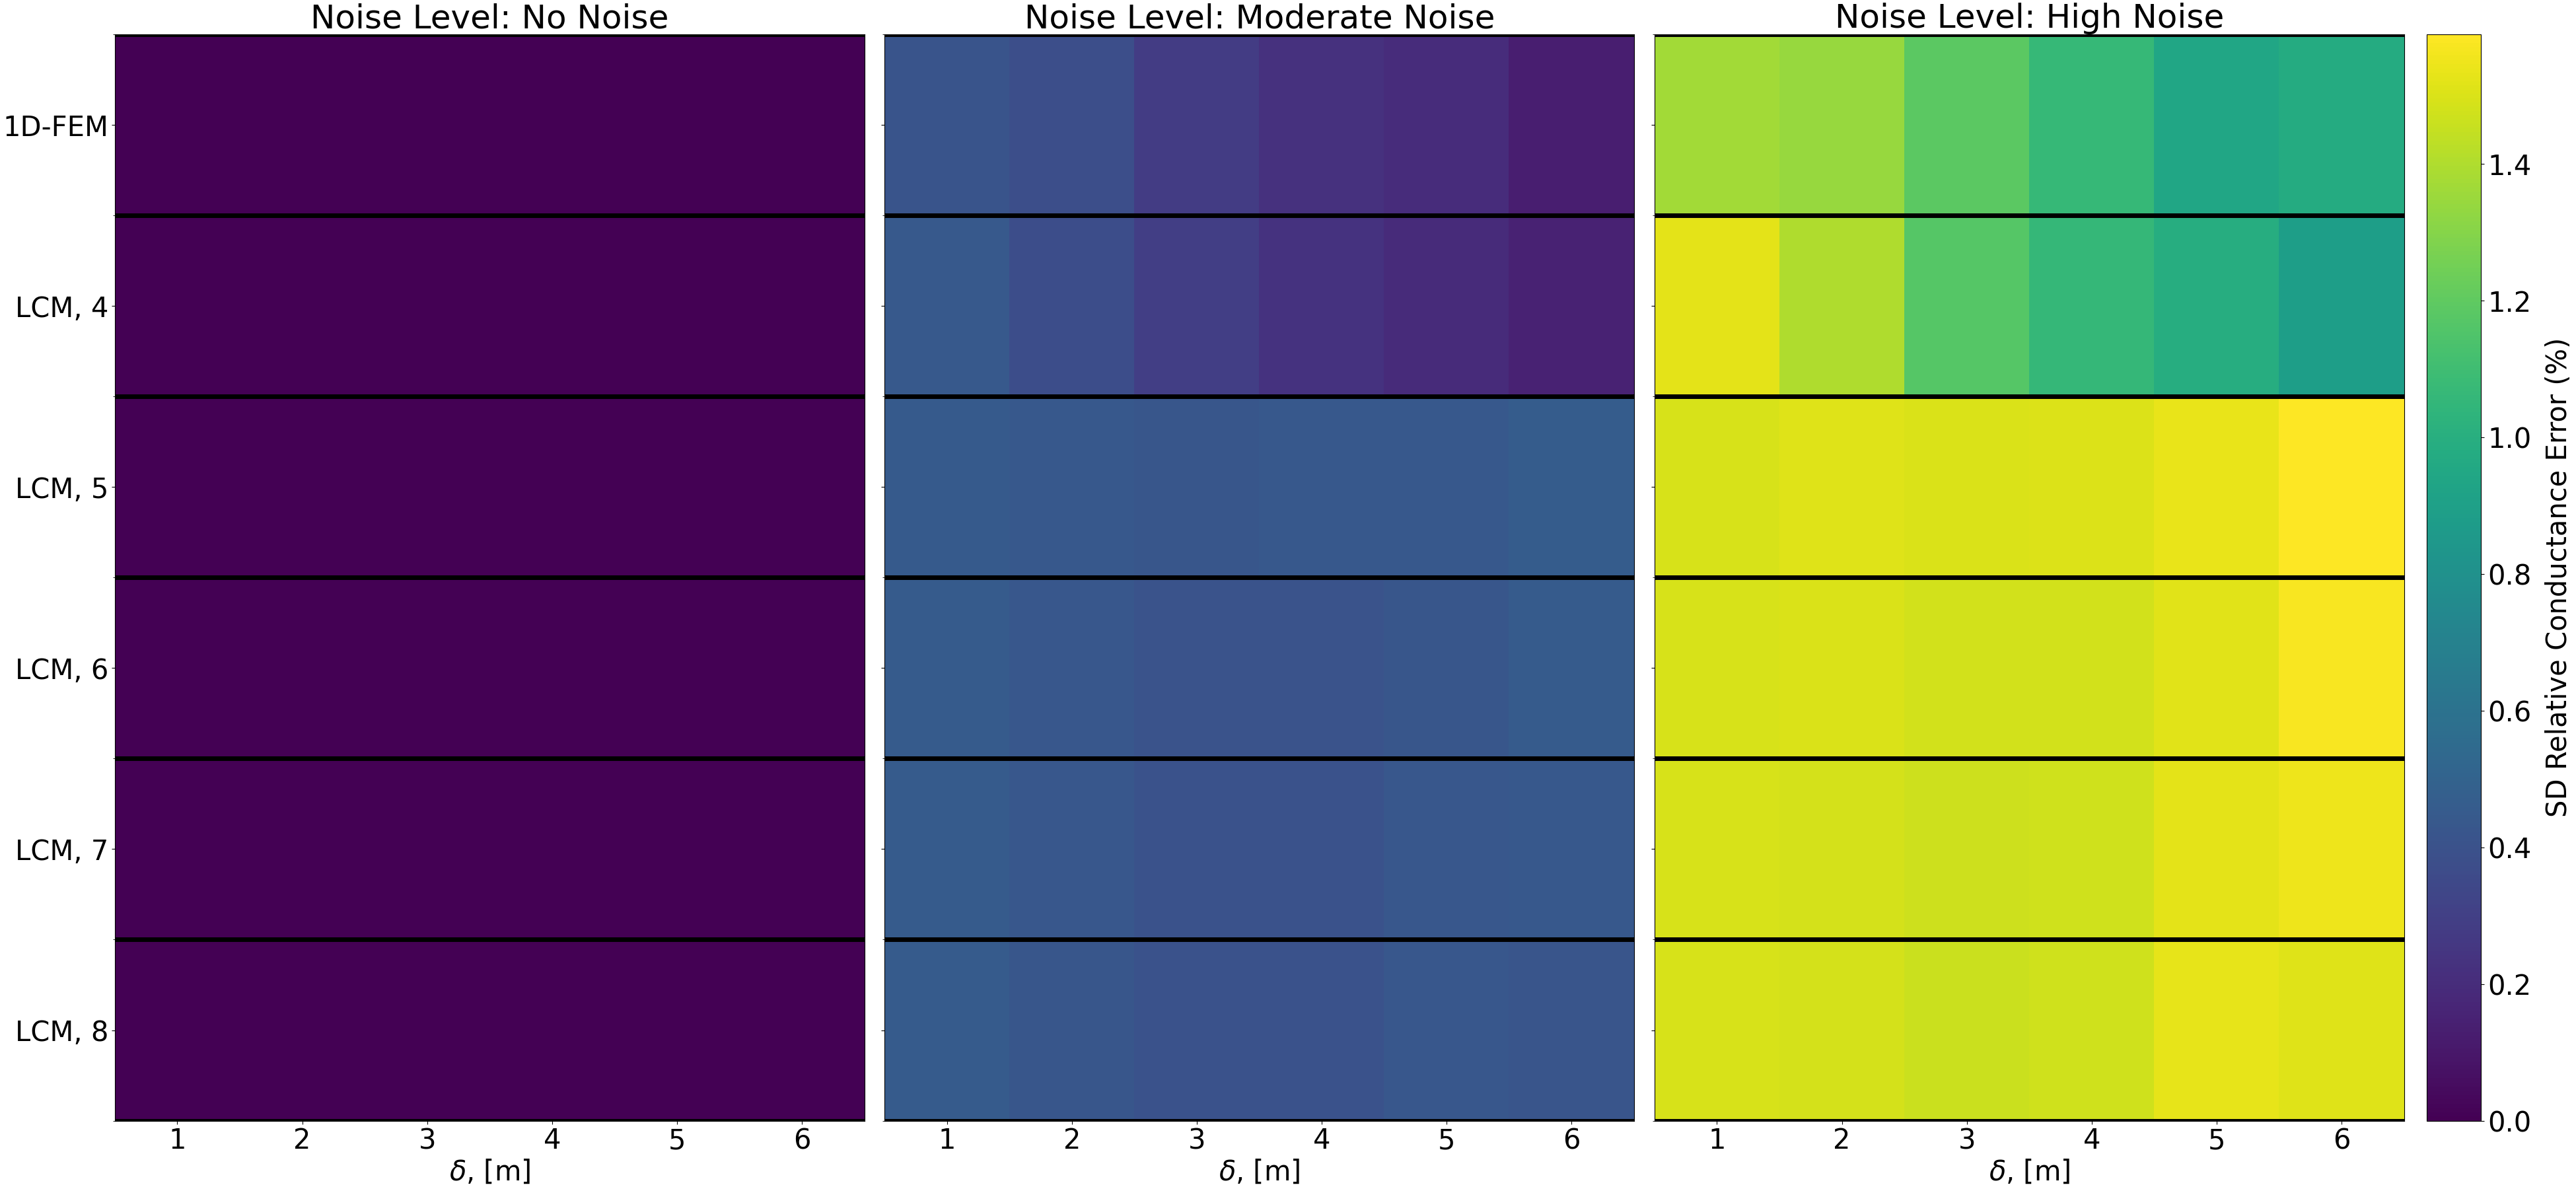
\includegraphics[width=0.99\textwidth]{./figs/results/cond_sd.png}
    \caption{The standard deviation of the relative error for the inferred conductance values from a range of experiments and model selections. }
    \label{fig:cond_std}
\end{figure}

\begin{enumerate}
    \item What model won? E.g. Model A with Noise B performed the best
    \item All else should perhaps be placed in the appendix, with this section only highlighting what model we will compare the PIROM to (to reduce total number of combinations and overall noise in the paper)
\end{enumerate}
\subsubsection{Model Performance on Transient-Dominated Timescale}

For the experiments conducted in the previous sections, the timescale was fixed and sufficiently long; in other words, the simulation time in which the models ran for was extensive enough to ensure the heat applied on the boundary condition was able to propagate through the entirety of the system. Through this, the inferred conductance inherently satisfies the steady-state effects, of whose error would dominate the cost function used to train. However, such a result brings to question the transient effects. When the timescale is short enough where the initial transients dominates --- that is, times where heat has not been able to fully penetrate the system --- the inferred conductances should have higher error as the system tries to compensate for effects it can not fully observe yet. 

Consider Fig.~\ref{fig:char_time}, which shows the error in each inferred conductance as the timescale of the simulation is altered. Observe that there is a certain simulation timescale in which the relative error drops below an adequately low threshold, which perfectly coincides with the effective characteristic time of each of the gaps. In other words, the error drops off the moment where the flux reaches the sensor located immediately after each of the respective gaps. This finding is meaningful; the time needed to infer the conductance of a gap is only the time it takes for heat to travel to the sensors on either side of the gap. Therefore, the framework does not directly necessitate steady-state, but merely must be able to observe the temperatures on either side of the gap to read the physics across it. 

For the remainder of the study, the timescale will remain adequately large to ensure sufficient heat penetration through the system; as the PIROM will mainly focus on improved tracking of sensor readings, its ability to improve transient and steady-state effects is non-trivial. However, through these results, the framework is proven capable of inferring material properties within significantly reduces timescales --- even ones which are still dominated by transients --- as long as there is observation on either side of the gap in question. 

\begin{figure}[htbp]
    \centering
    
\includegraphics[width=0.99\textwidth]{./figs/results/char_time.png}
    \caption{Evolution of error in inferred conductance as a function of simulation timescale.}
    \label{fig:char_time}
\end{figure}

\subsection{PIROM Results}
\subsubsection{PIROM Optimization}
\begin{enumerate}
    \item Hidden dynamics
    \item TCR
    \item Training costs
    \item Generalization (DONE BELOW)
    \item HS Graph??
\end{enumerate}



\subsubsection{BC Generalization}

For the nominal experiment, the boundary condition (i.e., the flux applied on the edge of the TPS) is constant throughout the simulation. However, in a real experiment, this is not always true; there are small fluctuations in the boundary conditions that the PIROM must continue to track. To do so, a sinusoidal contribution will be added to the forcing applied to the TPS. 

Consider the flux component applied to the edge of the TPS given by
\begin{equation}
    q = \sigma \cdot \left[1+\sin(\omega t)\right]
\end{equation}
where $\sigma$ and $\omega$ represent the magnitude and periodic frequency of the forcing respectively. Previously, $\omega$ is zero, signifying a constant signal. However, by randomly sampling $\omega$, a periodic element can perturb the signal while still maintaining grounding in the same general vicinity of the nominal forcing. 

The results of such perturbation are shown in Fig.~\ref{fig:track_err}, where the NRMSE of PIROM is quite significantly lower than that of both the LCM and FEM. This is an artifact of the improved tracking of the PIROM through the learned hidden states, which as expected, extend to other boundary conditions without further training. This is advantageous as only the nominal boundary conditions (i.e., constant flux) must be explicitly learned by PIROM, and the learned hidden states can be implicitly applied to any set of boundary conditions and show major improvement. A further advantage of this is warm starting; even if the error is not adequately low, it provides a much better starting point for training than cold starting would, significantly decreasing runtime for a subsequent training instance. 

\subsubsection{Material Generalization}

Another important application to test is material generalization. At high temperatures, material properties may carry more uncertainty and in practice, may not exactly match the properties that the PIROM was trained on. Thus, PIROM having the capability to extend to slightly perturbed properties is imperative in ensuring its improved tracking retains accuracy in high temperature supersonic environments. 

To model this, the material properties can be formulated as
\begin{equation}
    m^{(p)} (\bar{T}) = m^{(n)}(\bar{T}) + 0.5\Delta m^{(n)}\left[ \alpha_0 \bar{T} + \alpha_1 \sin(\alpha_2 \pi \bar{T})\right]
\end{equation}
where $m^{(p)}$ and $m^{(n)}$ are the perturbed and nominal material properties respectively, $\bar{T}$ is the normalized temperature given by $\bar{T} = \frac{T - T_\text{min}}{T_\text{max}-T_\text{min} }$, and $\xi = [\alpha_0, \alpha_1, \alpha_2]$ are the random parameters sampled to perturb the material properties.
Such a model succeeds in keeping material properties true at low temperatures, but allowing larger perturbations as temperature continues to climb. The generated perturbations are illustrated in Fig.~\ref{fig:pert_mats}, where sufficient deviation from the nominal properties is demonstrated. 

\begin{figure}[htbp]
    \centering
    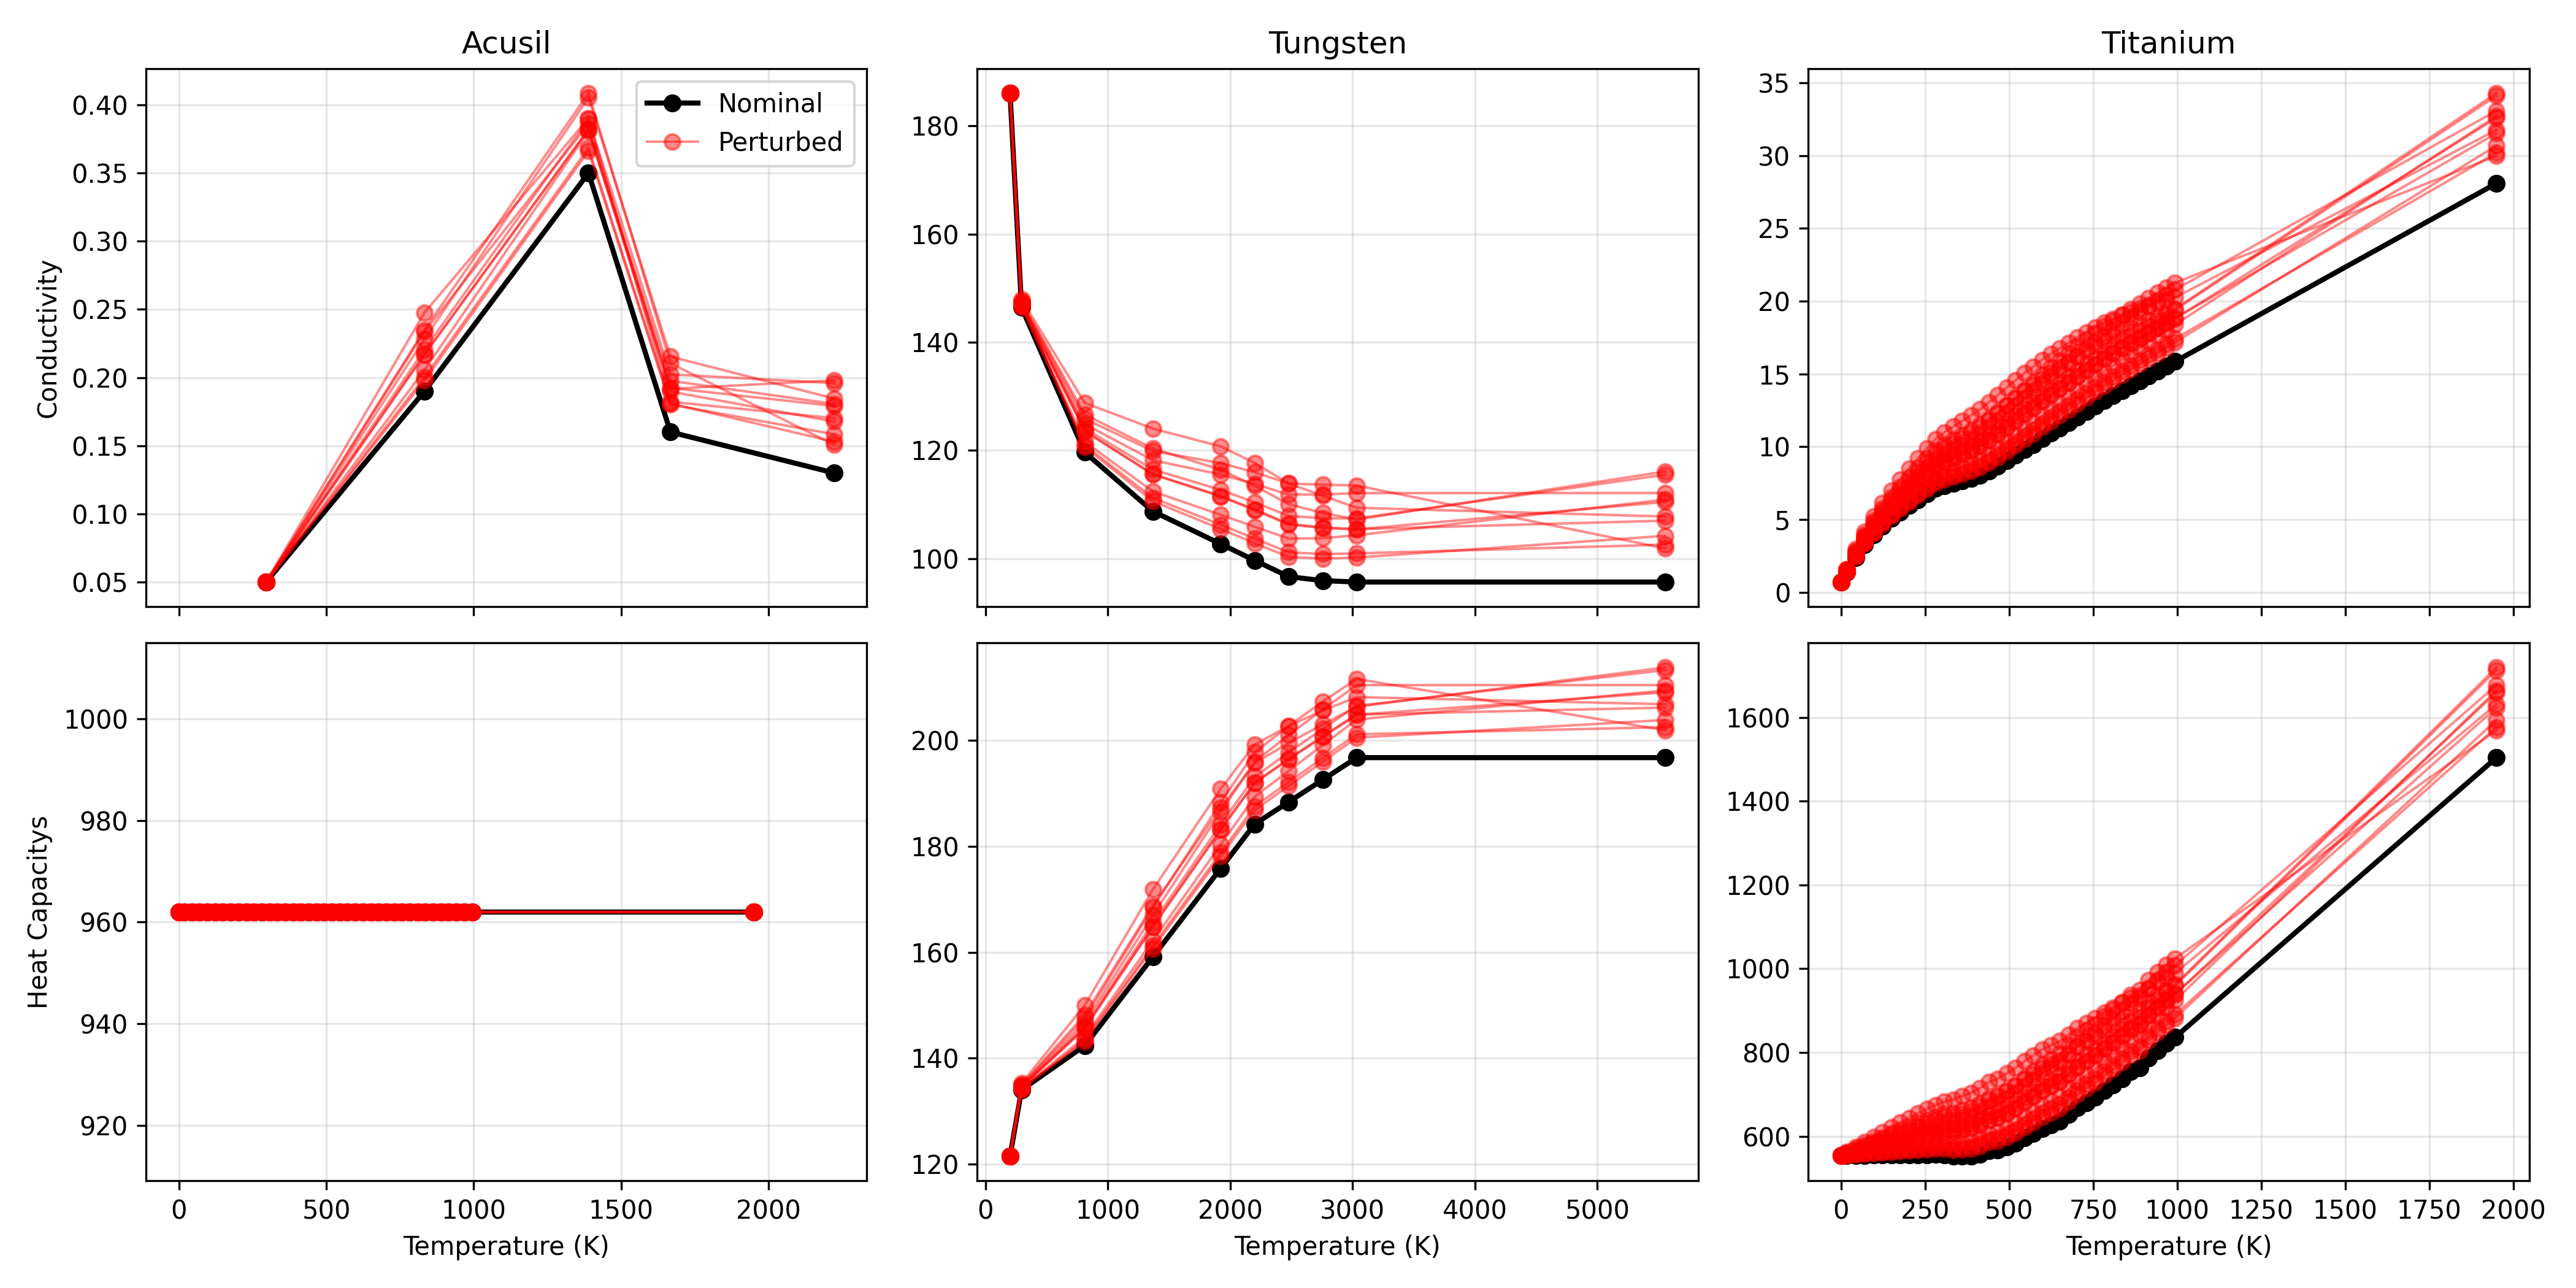
\includegraphics[width=0.9\textwidth]{./figs/modeling/pert_mats.png}
    \label{fig:pert_mats}
\end{figure}

\subsubsection{TCR Generalization}
\subsubsection{Thickness Generalization}
\subsubsection{Compounded Generalization}

\subsubsection{Extreme Thickness Generalization}

\begin{figure}[htbp]
    \centering
    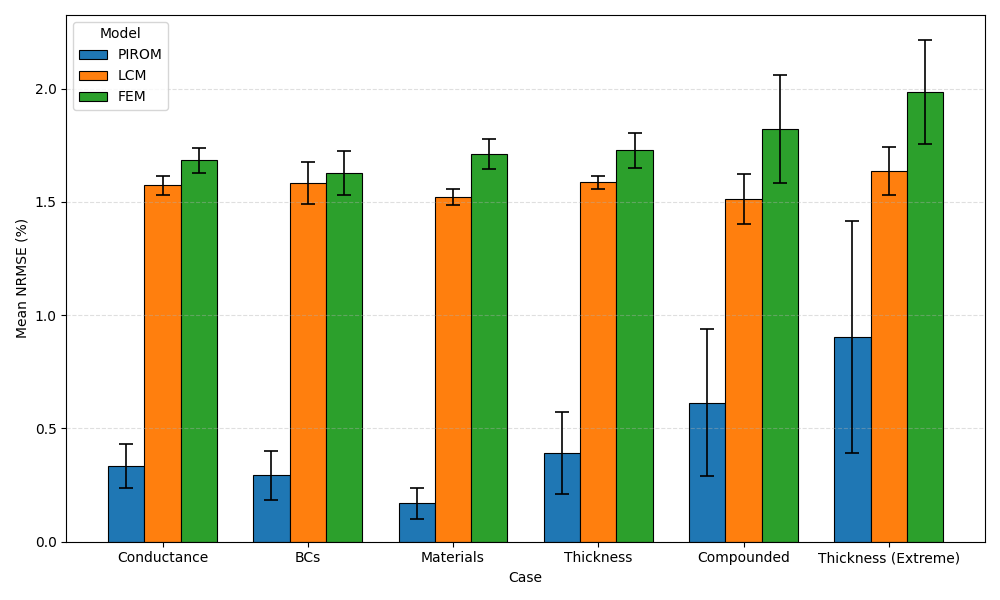
\includegraphics[width=0.9\textwidth]{./figs/results/tracking_error.png}
    \caption{Mean NRMSE of sensor tracking for each of the generalization cases. }
    \label{fig:track_err}
\end{figure}